\section{Consistency study}
In this section, we investigate the effect of changing
$\delta_{\rm sl}$ in the continuous, neutral model.
In all this section we will assume that
$z_0$ is constant.
The main direct changes when $\delta_{\rm sl}$ becomes
$\delta_{\rm sl}' < \delta_{\rm sl}$ are:
\begin{itemize}
\item the Coriolis effect and the large-scale forcing are
now taken into account for $z \in 
[\delta_{\rm sl}', \delta_{\rm sl}]$;
\item the viscosity $K(z)$ for $z \in 
[\delta_{\rm sl}', \delta_{\rm sl}]$ is not forced by the law
of the wall anymore.
\end{itemize}
There are also indirect effects due to the non-linearity of the
problem:
\begin{itemize}
	\item Even if the bulk algorithm is well designed and returns
		the same friction scales whether it takes as input
		$(\delta_1, u_2(\delta_1))$ or 
		$(\delta_2, u_2(\delta_2))$ (which is assumed to
		be the case),
		the input differs between $u_1$ and $u_2$ because
		of the direct effects.
\end{itemize}

\subsection{Study of the consistency: neutral case}
Let $\delta_1$,$\delta_2$ two
different heights of surface layer
such that $\delta_1 < \delta_2$.

Let $u_1$, $u_2$, be solutions of 
\eqref{eq:ND_NeutralCase_continuousModel} using
respectively $\delta_1, \delta_2$ for $\delta_{sl}$.

\subsubsection{Analytical study assuming identical viscosities}
First, note that inside the surface layer for $u_2$,
since $u_2(z) = \frac{u_\star}{\kappa}\log(1+\frac{z}{z_0})
\frac{u_2(\delta_{2})}{||u_2(\delta_{2})||}$, assuming
$||u_2(\delta_{2})||$ follows the same log low (it only works
when the problem is continuous in time)
\begin{equation}
(\partial_t + if) u_2(z) = \frac{\log(1+\frac{z}{z_0})}
{\log(1+\frac{\delta_2}{z_0})}(\partial_t + if) u_2(\delta_2), 
~~~\forall z \leq \delta_2
\end{equation}
Let us assume that $K\partial_z u_2$ is $C^1$ at $\delta_2$;
then $\partial_z (K\partial_z u_2) = 0$ in all the interval
$(0, \delta_2)$ and the evolution equation of $u_2$ in
$(\delta_1, \delta_2)$ is
\begin{equation}
(\partial_t + if) u_2(z) = \frac{\log(1+\frac{z}{z_0})}
{\log(1+\frac{\delta_2}{z_0})} i f u_G, 
	~~~\forall z \in (\delta_1, \delta_2).
\end{equation}
The difference between $u_1$ and $u_2$ is governed by this interval:
subtracting the two evolution equations gives
\begin{equation}
(\partial_t + if) (u_2 - u_1) = \left(\frac{\log(1+\frac{z}{z_0})}
{\log(1+\frac{\delta_2}{z_0})} - 1\right)i f u_G 
-
\partial_z (K \partial_z u_1), ~~~\forall z \in (\delta_1, \delta_2).
\end{equation}
We see in the right hand side of the latter equation the two items
of the beginning of the section:
the large-scale forcing with the Coriolis effect,
and the diffusion term of $u_1$ which is actually
$\partial_z (K \partial_z u_1) = \partial_z (K \partial_z u_1 - K \partial_z u_2)$

Let $w=u_2 - u_1$. If we assume that $K$ is the viscosity for both
$u_2$ and $u_1$ then
\begin{equation}
	\begin{cases}
		(\partial_t + if) w = \partial_z (K \partial_z w) ,
		~~ \forall z > \delta_2 \\
(\partial_t + if) w = \partial_z (K \partial_z w) + \left(\frac{\log(1+\frac{z}{z_0})}
{\log(1+\frac{\delta_2}{z_0})} - 1\right)i f u_G 
, ~~~\forall z \in (\delta_1, \delta_2) \\
		K \partial_z w = \frac{\kappa}
		{\log(1+\frac{\delta_1}{z_0})}\left(
		u_{\star, 2} u_2(\delta_1) -
		u_{\star, 1} u_1(\delta_1)\right),
		~~~ \forall z \leq \delta_1.
	\end{cases}
\end{equation}
Apart from the bulk sensitivity in the surface condition,
the difference is hence from the forcing
$\left(\frac{\log(1+\frac{z}{z_0})}
{\log(1+\frac{\delta_2}{z_0})} - 1\right)i f u_G$.
This forcing is more important when $\frac{\delta}{z_0}$
is small.
\subsubsection{Semi-Discrete Consistency (Finite Differences)}
This subsection shows that the semi-discrete in space
Finite Differences
scheme is not sensitive to the value of $\delta_{\rm sl}$.
We put aside the sensitivity of the bulk procedure by
assuming that $z_{0M}$ is a constant.
%
The approach used in Finite Differences consists in assuming
$\delta_{\rm sl} = z_{1/2}$ and to use the flux at $z_0$ in
the integration in time
$K_0\phi_0 = u_\star^2
\frac{u(\delta_{\rm sl})}{||u(\delta_{\rm sl})||}$
(we assume that $u(0)=0$ for simplicity).
We generalize the usual approach with
$\delta_{sl} = z_{1/2} - \epsilon$ with
$\epsilon < \frac{h_{\frac{1}{2}}}{2}$. 
The value $u(\delta_{\rm sl})$ can be approximated
by $u_{1/2} - (\partial_z u)(\delta_{\rm sl})\epsilon$.
The implementation of such a boundary condition would be
\begin{equation}
	\label{eq:ND_Consistency_SemiDiscreteBdCond}
K_0\phi_0 = 
\kappa^2 ||u_{1/2} - (\partial_z u)(\delta_{\rm sl})\epsilon ||
	\frac{u_{1/2} - (\partial_z u)(\delta_{\rm sl})\epsilon 
}{\log(1+\frac{\delta_{sl}}{z_{0M}})^2}
\end{equation}
and it becomes convenient to compute the difference between
$\delta_{sl}=z_{1/2}$ and $\delta_{sl}'=z_{1/2}-\epsilon$.
Indeed,
$|u - (\partial_z u) \epsilon| = |u| -
\epsilon \frac{\mathfrak{R}(\overline{u} \partial_z u)}{|u|}
+ O(\epsilon^2)$ so
$|u - (\partial_z u) \epsilon|(u - (\partial_z u) \epsilon) =
|u|u -
\epsilon \left(
u\frac{\mathfrak{R}(\overline{u} \partial_z u)}{|u|}
+ |u| \partial_z u
\right)
+ O(\epsilon^2)$.
Using the wall law
$\partial_z u=\frac{u(\delta_{\rm sl})}{(\delta_{\rm sl} + z_0)
\log(1+\frac{\delta_{sl}}{z_0})}$ we obtain 
\begin{equation}
|u - (\partial_z u) \epsilon|(u - (\partial_z u) \epsilon) - |u|u =
	- \epsilon \left(\frac{2|u_{1/2}|u_{1/2}}
	{(\delta_{\rm sl} + z_0) \log(1+\frac{\delta_{sl}}{z_0})}
	\right)+ O(\epsilon^2)
\end{equation}
Combining with $\frac{\kappa^2}{\log(1+\frac{\delta_{sl}}{z_0})}$,
we find the derivative of the right-hand side of
\eqref{eq:ND_Consistency_SemiDiscreteBdCond} with respect to
$\delta_{sl}$ to be equal to zero.
In conclusion, if $z_{0M}$ does not depend on $u$ and if
the evolution equation is integrated in time at $z_\frac{1}{2}$,
then for the Finite Differences scheme
\begin{equation}
	\partial_{\delta_{sl}} (K_0 \phi_0) = 0.
\end{equation}
This result is expected since in the boundary condition
$K_0 \phi_0 = u_\star^2 e_\tau$ the orientation $e_\tau$ is
not changed by the use of the wall law for $\partial_z u$
and the friction scale $u_\star$ is not affected because
$u(z_\frac{1}{2} - \epsilon)$ is given by the wall law.
\subsection{Study of the consistency: stable case}
We study numerically in a stable case the consistency of the
discretisations: how the change of the space step affects the
solution of the discrete equations ?
\paragraph{Description of the test case}
We intend to obtain a strongly stratified profile: the temperature
is hence increasing with the height at the initialization and
the surface temperature decreases with time.
The initial temperature is $265$ K in the first 100 meters of the
atmosphere and then gains 1 degree every 100 meters;
the surface temperature starts at 265 K and loses
1 degree every ten hours.
The geostrophic wind is $u_G = 8 \;{\rm m}.{\rm s}^{-1}$,
the time step is $\Delta t = 30 \;{\rm s}$.
\begin{figure}
	\centering
\includegraphics[scale=0.6]{images/Stratified.pdf}
	\caption{ Evolution of $u_\star$ and
		vertical profiles of $|u|$ and $\arg(u)$ for
		several surface flux schemes. Above 200m,
		the profiles are those of the initial condition.
	}
	\label{fig:ND_Consistency_Stratified}
\end{figure}
The profiles obtained after 72 hours of integration are
shown in Figure \ref{fig:ND_Consistency_Stratified}.
It is seen that the temperature and wind profiles are
all similar.
Two simulations are done: the first one uses 15 grid points
in the 400m column and the second one uses 40 grid points and is then
projected onto the first grid for the comparison.
\begin{figure}
	\centering
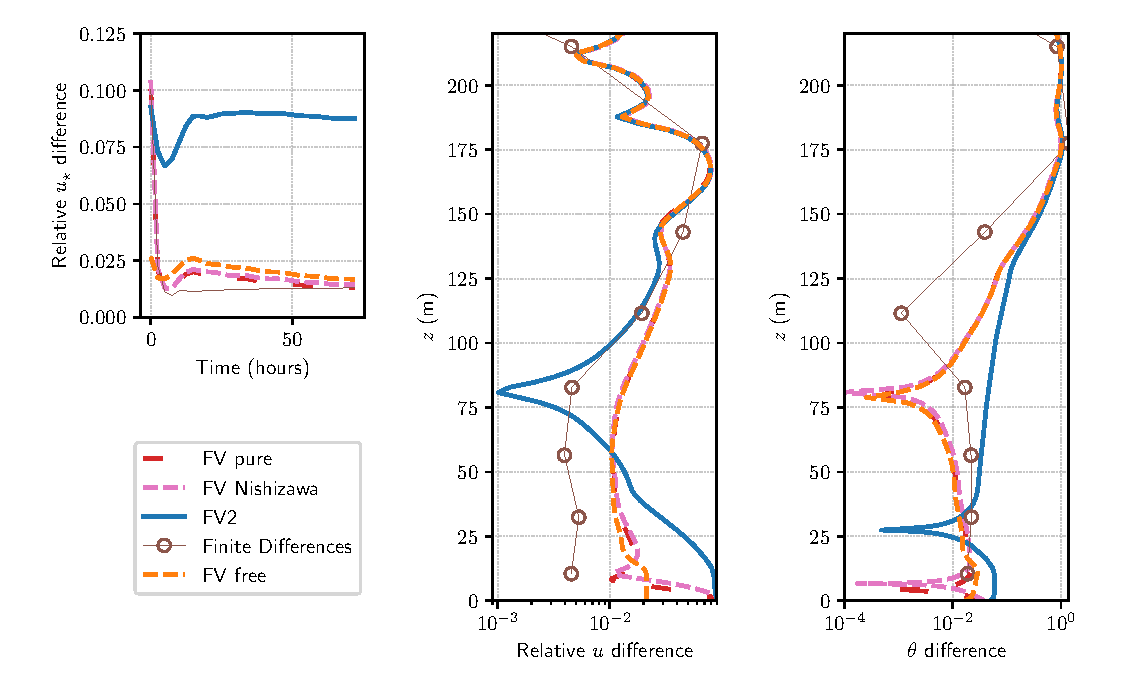
\includegraphics[scale=0.6]{images/consistency_comparisonStratified.pdf}
	\caption{Differences in $u_\star, |u|$ and $\arg(u)$
	between a high resolution and a low resolution
	of the surface flux schemes presented in a stable
	stratification.
	}
	\label{fig:ND_Consistency_comparisonStratified}
\end{figure}
\paragraph{Results} The differences between the two simulations are shown in Figure
\ref{fig:ND_Consistency_comparisonStratified}.
The difference between the high resolution and the low resolution
does not significantly change with the surface flux schemes.
The difference in $u_\star$ is especially high for the "FV2" scheme.
Note that the initialization for FV free and FV2 is particular:
to ensure the continuity of the solution,
the initial profile is already adjusted for the
MO theory. This is why the relative $u_\star$ difference is zero
at initialization whereas it is very high for the other surface flux
schemes.
%
The "FV2" scheme is not very consistent because it follows the
continuous model with $\delta_{sl}$ changing together with the
space step.
The Finite Differences method or the "FV pure" methods suffer
less from this problem because even if $\delta_{sl}$ changes,
it is assumed that the evolution equation is
integrated inside the surface layer.
\cite{maronga_improved_2020} also find that the
sensitivity of their LES model to the grid spacing is
"\textit{more
likely related to under-resolved near-surface gradients
and turbulent mixing at the boundary-layer top, to the
[sub-grid scale] model formulation, and/or to numerical issues,
and not to deficiencies due to the use of improper surface
boundary conditions}".
\subsection{Study of the consistency: unstable case}
\begin{figure}
	\centering
	\includegraphics[scale=0.6]{images/consistency_comparisonUnstable.pdf}
	\caption{Differences in $u_\star, t_\star, |u|$ and $\theta$
	between a high resolution and a low resolution
	of the surface flux schemes presented in an unstable
	stratification.
	}
	\label{fig:ND_Consistency_comparisonUnstable}
\end{figure}
Figure \ref{fig:ND_Consistency_comparisonUnstable}
shows the differences found between a high resolution simulation
and a low resolution simulation in an unstable situation.
\paragraph{Description of the test case}
To design a test case with an unstable stratification
the sea surface temperature is forced to follow a daily oscillation
between $279$ K and $281$ K.
The initial profiles of temperature and wind
are set to constant values of respectively $280$ K and
$8 \; {\rm m}.{\rm s}^{-1}$.
As in the stable case the geostrophic wind is
$u_G = 8 \;{\rm m}.{\rm s}^{-1}$
and the time step is $\Delta t = 30 \;{\rm s}$.
The "low resolution" is composed of 50 grid levels of $10 \; m$
each; 15 additional stretched levels between $500 \; m$ and
$1080 \; m$ make sure that the upper boundary condition
is not involved in the results.
The "high resolution" divides every space levels into
3 space levels of equal size.
\paragraph{Results}
Figure \ref{fig:ND_Consistency_comparisonUnstable}
shows that the "FV2" scheme is also less consistent
in the unstable case.
This time in the first $200$ meters the scheme "FV free" seems a lot
more robust than the other.
However, above this height the differences between the high
resolution and the low resolution simulations oscillate and there
is no clear conclusion that can be made.
As in the stable case, the schemes that assume an evolution equation
inside the surface layer are not very sensitive to the choice of
the height of the surface layer.
The main conclusion is hence that
\textbf{if Monin-Obukhov profiles are enforced in the
surface layer the importance of the choice of
$\delta_{sl}$ increases.}.
